% ==============================================================================
% MULTI_DATASET_SLIDES.tex
% Benchmarking Quantum Machine Learning in Diabetes Diagnostics:
% A Multi-Dataset Cross-Methodology Audit and Leakage Deconstruction
%
% 16:9 Widescreen Professional Beamer Deck (22 frames)
% Plain-language, highly visual, all abbreviations defined in small print.
% ==============================================================================
\documentclass[aspectratio=169,10pt,t,xcolor={table,dvipsnames}]{beamer}
\usetheme{Madrid}

% --- Typography and Math Packages ---
\usepackage[T1]{fontenc}
\usepackage{lmodern}
\usepackage{amsmath,amssymb,amsfonts}
\usepackage{booktabs,array,multirow}
\usepackage{graphicx}
\usepackage{adjustbox}
\usepackage{tikz}
\usetikzlibrary{positioning,arrows.meta,calc,shapes.geometric,fit}

% --- Custom Professional Palette ---
\definecolor{qnavy}{HTML}{0B2545}     % Primary Deep Navy
\definecolor{qteal}{HTML}{134E5E}     % Secondary Slate Teal
\definecolor{qcrimson}{HTML}{B91C1C}  % Warning / Alert Crimson
\definecolor{qgreen}{HTML}{15803D}   % Success / Verified Forest Green
\definecolor{qamber}{HTML}{B45309}   % Caution / Highlight Amber
\definecolor{qslate}{HTML}{475569}   % Cool Slate Gray
\definecolor{qlight}{HTML}{F8FAFC}   % Neutral Light Background
\definecolor{qcard}{HTML}{EEF2F6}    % Card Background

\definecolor{qcrimsonbg}{HTML}{FDF2F2} % Light crimson tint for alerted blocks
\definecolor{qgreenbg}{HTML}{F0FDF4}   % Light green tint for example blocks

% --- Beamer Styling Overrides ---
\setbeamercolor{structure}{fg=qnavy}
\setbeamercolor{palette primary}{bg=qnavy,fg=white}
\setbeamercolor{palette secondary}{bg=qteal,fg=white}
\setbeamercolor{palette tertiary}{bg=qnavy,fg=white}
\setbeamercolor{frametitle}{bg=qnavy,fg=white}
\setbeamercolor{title}{bg=qnavy,fg=white}

\setbeamercolor{block title}{bg=qnavy,fg=white}
\setbeamercolor{block body}{bg=qcard,fg=black}
\setbeamercolor{block title alerted}{bg=qcrimson,fg=white}
\setbeamercolor{block body alerted}{bg=qcrimsonbg,fg=black}
\setbeamercolor{block title example}{bg=qgreen,fg=white}
\setbeamercolor{block body example}{bg=qgreenbg,fg=black}

\setbeamercolor{item}{fg=qteal}
\setbeamertemplate{navigation symbols}{}
\setbeamertemplate{blocks}[rounded][shadow=false]
\setbeamertemplate{itemize items}[circle]
\setbeamertemplate{enumerate items}[default]
\setbeamerfont{frametitle}{size=\large,series=\bfseries}
\setbeamertemplate{caption}{\raggedright\scriptsize\insertcaption\par}

% --- Custom Header & Footline (Fixed: Zero nullfont warnings) ---
\setbeamertemplate{footline}{%
  \leavevmode%
  \hbox{%
  \begin{beamercolorbox}[wd=.35\paperwidth,ht=2.5ex,dp=1.1ex,left,leftskip=1em]{palette primary}%
    \normalfont\scriptsize\bfseries Clinical QML Multi-Dataset Audit%
  \end{beamercolorbox}%
  \begin{beamercolorbox}[wd=.45\paperwidth,ht=2.5ex,dp=1.1ex,center]{palette secondary}%
    \normalfont\scriptsize\insertshorttitle%
  \end{beamercolorbox}%
  \begin{beamercolorbox}[wd=.20\paperwidth,ht=2.5ex,dp=1.1ex,right,rightskip=1em]{palette primary}%
    \normalfont\scriptsize\bfseries\insertframenumber{} / \inserttotalframenumber%
  \end{beamercolorbox}}%
  \vskip0pt%
}

% --- Custom Badges and Highlights ---
\newcommand{\cmark}{\textcolor{qgreen}{\textbf{\checkmark}}}
\newcommand{\xmark}{\textcolor{qcrimson}{\textbf{\texttimes}}}
\newcommand{\cval}[1]{\textcolor{qnavy}{\textbf{#1}}}
\newcommand{\bval}[1]{\textcolor{qcrimson}{\textbf{#1}}}
\newcommand{\gval}[1]{\textcolor{qgreen}{\textbf{#1}}}
\newcommand{\pAbig}{\Large\bfseries}

% --- Plain-English Footnotes on each frame ---
\newcommand{\pfoot}[1]{\vfill{\raggedright\tiny\color{qslate}#1\par}}

% --- Visual Card Styles ---
\tikzset{
  pAcard/.style={draw=#1,fill=#1!8,rounded corners=4pt,line width=1pt,inner sep=4pt,text width=6.55cm,minimum height=2.2cm,anchor=north west,align=left,font=\scriptsize},
  pAbx/.style={draw=#1,fill=#1!10,rounded corners=3pt,inner sep=4pt},
  pAbxW/.style={draw=#1,fill=#1!10,rounded corners=3pt,inner sep=4pt,line width=0.8pt,minimum width=3.3cm,minimum height=0.7cm},
  pAbxT/.style={draw=#1,fill=#1!10,rounded corners=3pt,inner sep=4pt,text width=4.0cm,align=center},
  pAbxL/.style={draw=#1,fill=#1!10,rounded corners=3pt,inner sep=4pt,text width=7.6cm,align=left,anchor=north west}
}

% --- Color key for table cells ---
\providecommand{\cbaC}[1]{%
  \ifdim#1pt<0.55pt\cellcolor{qcrimson!30}\else
  \ifdim#1pt<0.65pt\cellcolor{qamber!35}\else
  \ifdim#1pt<0.80pt\cellcolor{qamber!12}\else
  \ifdim#1pt<0.88pt\cellcolor{qgreen!20}\else\cellcolor{qgreen!38}\fi\fi\fi\fi#1}
\providecommand{\tlC}[1]{\tikz[baseline=-0.6ex]\fill[#1] (0,0) circle (0.11);}

% --- Image Search Paths ---
\graphicspath{{figures/}{gen_v2/}{../figures/}}

% --- Presentation Metadata ---
\title[Do Quantum Models Help Diagnose Diabetes?]{Do Quantum Models Help Diagnose Diabetes?}
\subtitle{A Multi-Dataset Cross-Methodology Audit and Leakage Deconstruction}
\author[Independent Research Audit]{Senior ML Research Engineer \& Independent Audit Team}
\institute{Repository: \texttt{Adaptive-Quantum-Kernel-Selection}}
\date{November 2026}

\begin{document}

% ==============================================================================
% SLIDE 1: Title Slide
% ==============================================================================
\begin{frame}[plain]
  \vspace{0.6cm}
  \begin{center}
    {\usebeamercolor[fg]{structure}\LARGE\bfseries Do Quantum Models Help\\Diagnose Diabetes?\par}
    \vspace{0.2cm}
    {\large\color{qteal}\bfseries An independent check of 8 published studies on 4 diabetes datasets\par}
    \vspace{0.35cm}
    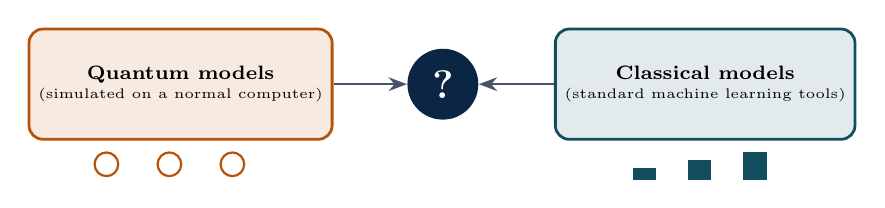
\begin{tikzpicture}[font=\scriptsize\bfseries,every node/.style={align=center}]
      \node[draw=qamber,fill=qamber!12,rounded corners=5pt,minimum width=3.8cm,minimum height=1.4cm,line width=1pt](q){Quantum models\\[-1pt]{\tiny\mdseries (simulated on a normal computer)}};
      \node[draw=qteal,fill=qteal!12,rounded corners=5pt,minimum width=3.8cm,minimum height=1.4cm,right=2.8cm of q,line width=1pt](c){Classical models\\[-1pt]{\tiny\mdseries (standard machine learning tools)}};
      \node[circle,fill=qnavy,text=white,font=\Large\bfseries,minimum size=0.9cm](mid) at ($(q)!0.5!(c)$){?};
      \draw[-{Stealth},thick,qslate](q.east)--(mid.west);
      \draw[-{Stealth},thick,qslate](c.west)--(mid.east);
      \foreach \i in {0,1,2}{\draw[qamber,thick]($(q.south west)+(1.0+0.8*\i,-0.3)$)circle(0.15);}
      \foreach \i/\h in {0/0.15,1/0.25,2/0.35}{\fill[qteal]($(c.south west)+(1.0+0.7*\i,-0.5)$)rectangle++(0.3,\h);}
    \end{tikzpicture}\par
    \vspace{0.5cm}
    {\scriptsize Independent re-implementation and verification. All numbers come from our executed benchmark results.\par}
    {\tiny November 2026 $\;\vert\;$ Repository: \texttt{Adaptive-Quantum-Kernel-Selection}\par}
  \end{center}
\end{frame}

% ==============================================================================
% SLIDE 2: Four Main Findings
% ==============================================================================
\begin{frame}{Four Main Findings}
  \centering
  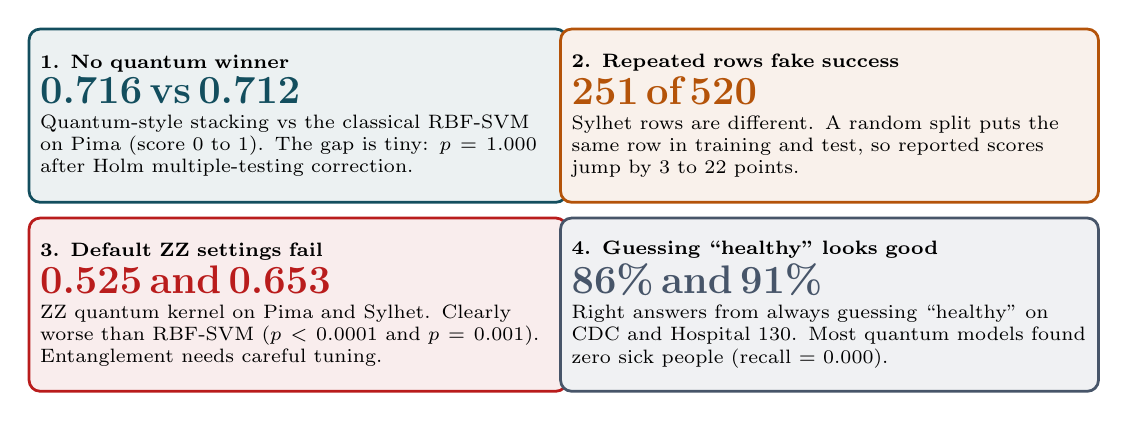
\begin{tikzpicture}[x=1cm,y=1cm]
    \node[pAcard=qteal](a) at (0,0){\textbf{1. No quantum winner}\\[1pt]\textcolor{qteal}{\pAbig 0.716 vs 0.712}\\[1pt]Quantum-style stacking vs the classical RBF-SVM on Pima (score 0 to 1). The gap is tiny: $p=1.000$ after Holm multiple-testing correction.};
    \node[pAcard=qamber](b) at (6.75,0){\textbf{2. Repeated rows fake success}\\[1pt]\textcolor{qamber}{\pAbig 251 of 520}\\[1pt]Sylhet rows are different. A random split puts the same row in training and test, so reported scores jump by 3 to 22 points.};
    \node[pAcard=qcrimson](c) at (0,-2.4){\textbf{3. Default ZZ settings fail}\\[1pt]\textcolor{qcrimson}{\pAbig 0.525 and 0.653}\\[1pt]ZZ quantum kernel on Pima and Sylhet. Clearly worse than RBF-SVM ($p<0.0001$ and $p=0.001$). Entanglement needs careful tuning.};
    \node[pAcard=qslate](d) at (6.75,-2.4){\textbf{4. Guessing ``healthy'' looks good}\\[1pt]\textcolor{qslate}{\pAbig 86\% and 91\%}\\[1pt]Right answers from always guessing ``healthy'' on CDC and Hospital 130. Most quantum models found zero sick people (recall = 0.000).};
  \end{tikzpicture}
  \pfoot{RBF-SVM = radial basis function support vector machine (classical). ZZ = quantum feature map built from two-qubit phase rotations. CDC = US Centers for Disease Control health survey. $p$ = statistical significance (small = real gap). Holm = multiple testing correction. Pima = diabetes laboratory study; Sylhet = early-stage symptom survey.}
\end{frame}

% ==============================================================================
% SLIDE 3: Why Diabetes Data?
% ==============================================================================
\begin{frame}{Why Diabetes Data?}
  \centering
  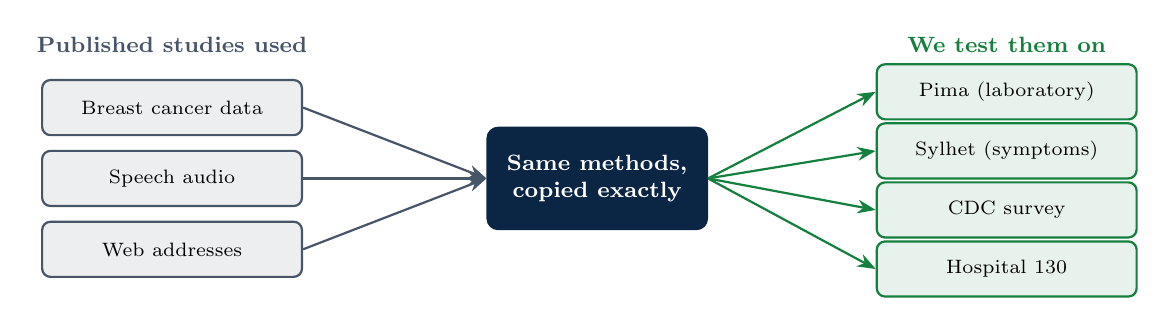
\begin{tikzpicture}[font=\scriptsize,every node/.style={align=center}]
    \node[font=\footnotesize\bfseries,text=qslate] at (0,2.3){Published studies used};
    \node[pAbxW=qslate](s1) at (0,1.5){Breast cancer data};
    \node[pAbxW=qslate](s2) at (0,0.6){Speech audio};
    \node[pAbxW=qslate](s3) at (0,-0.3){Web addresses};
    \node[draw=qnavy,fill=qnavy,text=white,rounded corners=4pt,minimum width=2.8cm,minimum height=1.3cm,font=\footnotesize\bfseries](m) at (5.4,0.6){Same methods,\\copied exactly};
    \node[font=\footnotesize\bfseries,text=qgreen] at (10.6,2.3){We test them on};
    \node[pAbxW=qgreen](d1) at (10.6,1.7){Pima (laboratory)};
    \node[pAbxW=qgreen](d2) at (10.6,0.95){Sylhet (symptoms)};
    \node[pAbxW=qgreen](d3) at (10.6,0.2){CDC survey};
    \node[pAbxW=qgreen](d4) at (10.6,-0.55){Hospital 130};
    \foreach \s in {s1,s2,s3}{\draw[-{Stealth},thick,qslate](\s.east)--(m.west);}
    \foreach \d in {d1,d2,d3,d4}{\draw[-{Stealth},thick,qgreen](m.east)--(\d.west);}
  \end{tikzpicture}\\[6pt]
  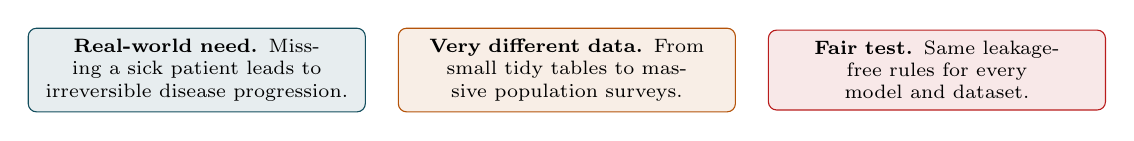
\begin{tikzpicture}[font=\scriptsize]
    \node[pAbxT=qteal]{\textbf{Real-world need.} Missing a sick patient leads to irreversible disease progression.};
    \node[pAbxT=qamber] at (4.7,0){\textbf{Very different data.} From small tidy tables to massive population surveys.};
    \node[pAbxT=qcrimson] at (9.4,0){\textbf{Fair test.} Same leakage-free rules for every model and dataset.};
  \end{tikzpicture}
  \pfoot{CDC = US Centers for Disease Control survey. Pima = classic female diabetes dataset ($N=768$). Sylhet = early-stage diabetes questionnaire ($N=520$). Hospital 130 = inpatient readmission database ($N=2{,}000$). Non-diabetes datasets (cancer, speech, URLs) were purged to maintain clinical focus.}
\end{frame}

% ==============================================================================
% SLIDE 4: The Four Datasets
% ==============================================================================
\begin{frame}{The Four Clinical Diabetes Datasets}
  \centering
  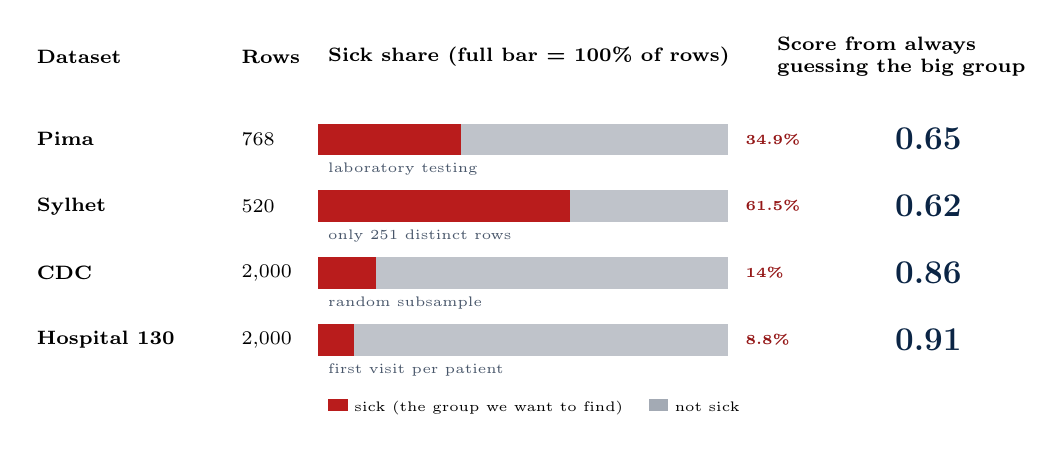
\begin{tikzpicture}[font=\scriptsize]
    \node[anchor=west,font=\scriptsize\bfseries] at (0,0.3){Dataset};
    \node[anchor=west,font=\scriptsize\bfseries] at (2.6,0.3){Rows};
    \node[anchor=west,font=\scriptsize\bfseries] at (3.7,0.3){Sick share (full bar = 100\% of rows)};
    \node[anchor=west,font=\scriptsize\bfseries,align=left] at (9.4,0.3){Score from always\\guessing the big group};
    \foreach \n/\r/\p/\f/\note [count=\i] in {Pima/768/34.9/0.65/{laboratory testing},Sylhet/520/61.5/0.62/{only 251 distinct rows},CDC/{2,000}/14/0.86/{random subsample},Hospital 130/{2,000}/8.8/0.91/{first visit per patient}}{
      \pgfmathsetmacro{\y}{-0.85*\i+0.1}
      \pgfmathsetmacro{\w}{5.2*\p/100}
      \node[anchor=west,font=\scriptsize\bfseries] at (0,\y){\n};
      \node[anchor=west] at (2.6,\y){\r};
      \fill[qcrimson](3.7,\y-0.2)rectangle({3.7+\w},\y+0.2);
      \fill[qslate!35]({3.7+\w},\y-0.2)rectangle(8.9,\y+0.2);
      \node[anchor=west,font=\tiny\bfseries,text=qcrimson!80!black] at (9.0,\y){\p\%};
      \node[anchor=west,font=\tiny,text=qslate] at (3.7,\y-0.38){\note};
      \node[anchor=west,font=\large\bfseries,text=qnavy] at (10.9,\y){\f};
    }
    \node[anchor=west,font=\tiny] at (3.7,-4.15){\textcolor{qcrimson}{\rule{0.25cm}{0.15cm}} sick (the group we want to find) \quad \textcolor{qslate!50}{\rule{0.25cm}{0.15cm}} not sick};
  \end{tikzpicture}
  \pfoot{CDC = US Centers for Disease Control health survey (self-reported diabetes/prediabetes). Pima = female diabetes testing. Sylhet = early-stage diabetes questionnaire. Hospital 130 = inpatient records (readmission within 30 days). Big group guessing accuracy = majority class baseline floor.}
\end{frame}

% ==============================================================================
% SLIDE 5: How to Read the Scores
% ==============================================================================
\begin{frame}{How to Read the Scores}
  \begin{columns}[T]
    \column{0.36\textwidth}
      \centering
      {\scriptsize\textbf{100 people (CDC-like: 14 sick)}}\\[3pt]
      
\begin{tikzpicture}[x=0.3cm,y=0.3cm]
        \foreach \i in {0,...,99}{
          \pgfmathtruncatemacro{\cx}{mod(\i,10)}
          \pgfmathtruncatemacro{\cy}{int(\i/10)}
          \ifnum\i<14 \fill[qcrimson](\cx,-\cy)circle(0.4);
          \else \fill[qslate!40](\cx,-\cy)circle(0.4);\fi}
      \end{tikzpicture}\\[3pt]
      {\tiny \textcolor{qcrimson}{$\bullet$} sick \quad \textcolor{qslate!60}{$\bullet$} healthy}
    \column{0.62\textwidth}
      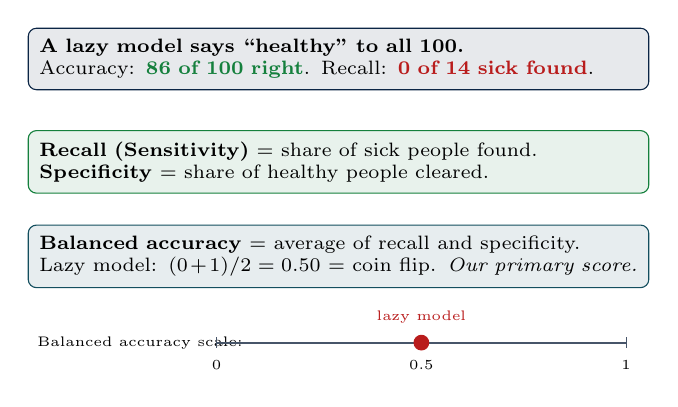
\begin{tikzpicture}[font=\scriptsize]
        \node[pAbxL=qnavy] at (0,0){\textbf{A lazy model says ``healthy'' to all 100.}\\ Accuracy: \gval{86 of 100 right}. Recall: \bval{0 of 14 sick found}.};
        \node[pAbxL=qgreen] at (0,-1.3){\textbf{Recall (Sensitivity)} = share of sick people found.\\ \textbf{Specificity} = share of healthy people cleared.};
        \node[pAbxL=qteal] at (0,-2.5){\textbf{Balanced accuracy} = average of recall and specificity.\\ Lazy model: $(0+1)/2=0.50$ = coin flip. \textit{Our primary score.}};
        \node[anchor=west,font=\tiny] at (0,-4.0){Balanced accuracy scale:};
        \draw[qslate,thick](2.4,-4.0)--(7.6,-4.0);
        \foreach \v in {0,0.5,1}{\draw[qslate]({2.4+5.2*\v},-3.93)--({2.4+5.2*\v},-4.07);\node[font=\tiny,anchor=north] at ({2.4+5.2*\v},-4.1){\v};}
        \fill[qcrimson]({2.4+5.2*0.5},-4.0)circle(0.1);
        \node[font=\tiny,text=qcrimson,anchor=south] at ({2.4+5.2*0.5},-3.88){lazy model};
      \end{tikzpicture}
  \end{columns}
  \pfoot{CDC = US Centers for Disease Control survey. On imbalanced data, 86\% accuracy is trivial (predicting majority). Balanced accuracy treats sick and healthy people equally; 0.50 is pure chance and 1.00 is perfect.}
\end{frame}

% ==============================================================================
% SLIDE 6: Claims That Do Not Add Up
% ==============================================================================
\begin{frame}{Claims That Do Not Add Up}
  \centering
  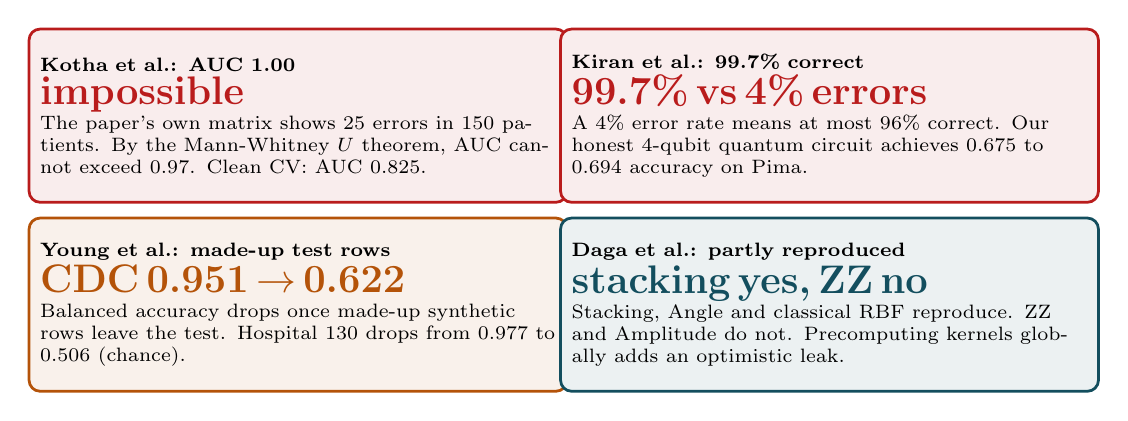
\begin{tikzpicture}[x=1cm,y=1cm]
    \node[pAcard=qcrimson](a) at (0,0){\textbf{Kotha et al.: AUC 1.00}\\[1pt]\textcolor{qcrimson}{\pAbig impossible}\\[1pt]The paper's own matrix shows 25 errors in 150 patients. By the Mann-Whitney $U$ theorem, AUC cannot exceed 0.97. Clean CV: AUC 0.825.};
    \node[pAcard=qcrimson](b) at (6.75,0){\textbf{Kiran et al.: 99.7\% correct}\\[1pt]\textcolor{qcrimson}{\pAbig 99.7\% vs 4\% errors}\\[1pt]A 4\% error rate means at most 96\% correct. Our honest 4-qubit quantum circuit achieves 0.675 to 0.694 accuracy on Pima.};
    \node[pAcard=qamber](c) at (0,-2.4){\textbf{Young et al.: made-up test rows}\\[1pt]\textcolor{qamber}{\pAbig CDC 0.951 $\to$ 0.622}\\[1pt]Balanced accuracy drops once made-up synthetic rows leave the test. Hospital 130 drops from 0.977 to 0.506 (chance).};
    \node[pAcard=qteal](d) at (6.75,-2.4){\textbf{Daga et al.: partly reproduced}\\[1pt]\textcolor{qteal}{\pAbig stacking yes, ZZ no}\\[1pt]Stacking, Angle and classical RBF reproduce. ZZ and Amplitude do not. Precomputing kernels globally adds an optimistic leak.};
  \end{tikzpicture}
  \pfoot{AUC = area under the receiver operating characteristic curve (1.0 = perfect ranking, 0.5 = random). CV = cross-validation. RBF = radial basis function. ZZ, Angle, Amplitude = quantum feature encodings. Stacking = meta-learner combining multiple model predictions.}
\end{frame}

% ==============================================================================
% SLIDE 7: Paper-Style Test vs Clean Test
% ==============================================================================
\begin{frame}{Paper-Style Test vs Clean Test}
  \centering
  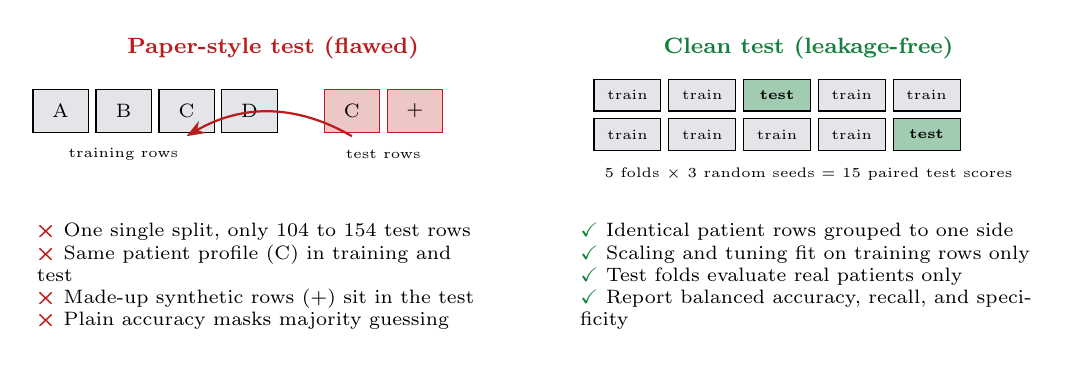
\begin{tikzpicture}[font=\scriptsize,every node/.style={align=center}]
    \node[font=\footnotesize\bfseries,text=qcrimson] at (3.2,0.4){Paper-style test (flawed)};
    \foreach \i/\t in {0/A,1/B,2/C,3/D}{\node[draw,fill=qslate!15,minimum width=0.7cm,minimum height=0.55cm] at (0.5+0.8*\i,-0.4){\t};}
    \node[draw=qcrimson,fill=qcrimson!25,minimum width=0.7cm,minimum height=0.55cm] at (4.2,-0.4){C};
    \node[draw=qcrimson,fill=qcrimson!25,minimum width=0.7cm,minimum height=0.55cm] at (5.0,-0.4){+};
    \node[font=\tiny] at (1.3,-0.95){training rows};
    \node[font=\tiny] at (4.6,-0.95){test rows};
    \draw[qcrimson,thick,-{Stealth}](4.2,-0.72)to[bend left=-30](2.1,-0.72);
    \node[text width=5.8cm,align=left] at (3.1,-2.5){\xmark\ One single split, only 104 to 154 test rows\\\xmark\ Same patient profile (C) in training and test\\\xmark\ Made-up synthetic rows (+) sit in the test\\\xmark\ Plain accuracy masks majority guessing};
    \node[font=\footnotesize\bfseries,text=qgreen] at (10.0,0.4){Clean test (leakage-free)};
    \foreach \i/\a in {0/train,1/train,2/test,3/train,4/train}{\node[draw,minimum width=0.85cm,minimum height=0.4cm,fill=qslate!15,font=\tiny] at (7.7+0.95*\i,-0.2){\a};}
    \foreach \i/\a in {0/train,1/train,2/train,3/train,4/test}{\node[draw,minimum width=0.85cm,minimum height=0.4cm,fill=qslate!15,font=\tiny] at (7.7+0.95*\i,-0.7){\a};}
    \fill[qgreen!40](7.7+1.9-0.425,-0.4)rectangle++(0.85,0.4);\draw(7.7+1.9-0.425,-0.4)rectangle++(0.85,0.4);
    \node[font=\tiny\bfseries] at (7.7+1.9,-0.2){test};
    \fill[qgreen!40](7.7+3.8-0.425,-0.9)rectangle++(0.85,0.4);\draw(7.7+3.8-0.425,-0.9)rectangle++(0.85,0.4);
    \node[font=\tiny\bfseries] at (7.7+3.8,-0.7){test};
    \node[font=\tiny] at (10.0,-1.2){5 folds $\times$ 3 random seeds = 15 paired test scores};
    \node[text width=5.8cm,align=left] at (10.0,-2.5){\cmark\ Identical patient rows grouped to one side\\\cmark\ Scaling and tuning fit on training rows only\\\cmark\ Test folds evaluate real patients only\\\cmark\ Report balanced accuracy, recall, and specificity};
  \end{tikzpicture}
  \pfoot{Fold = one of 5 equal splits; each split is held out as the test set once. Seed = random number generator starting value (repeated over 3 seeds for 15 runs). Grouped cross-validation ensures duplicate patient symptom profiles never span train and test.}
\end{frame}

% ==============================================================================
% SLIDE 8: Finding 1: Repeated Rows Inflate Scores
% ==============================================================================
\begin{frame}{Finding 1: Repeated Rows Inflate Scores on Sylhet}
  \begin{columns}[T]
    \column{0.42\textwidth}
      \centering
      {\scriptsize\textbf{Sylhet: 51.7\% of rows are copies}}\\[2pt]
      
\begin{tikzpicture}
        \pgfmathsetmacro{\sylw}{5.4*251/520}
        \fill[qgreen](0,0)rectangle(\sylw,0.45);
        \fill[qcrimson!70](\sylw,0)rectangle(5.4,0.45);
        \node[text=white,font=\scriptsize\bfseries] at (\sylw/2,0.22){251 unique};
        \node[text=white,font=\scriptsize\bfseries] at ({(\sylw+5.4)/2},0.22){269 copies};
        \node[font=\tiny] at (2.7,-0.2){520 total questionnaire rows};
      \end{tikzpicture}\\[6pt]
      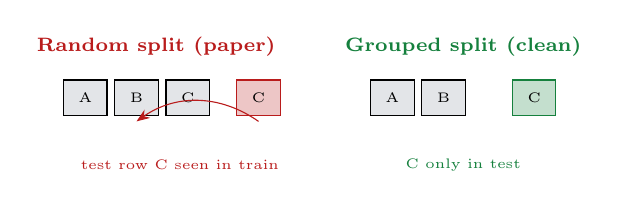
\begin{tikzpicture}[font=\tiny,every node/.style={align=center}]
        \node[font=\scriptsize\bfseries,text=qcrimson] at (1.3,1.0){Random split (paper)};
        \foreach \i/\t in {0/A,1/B,2/C}{\node[draw,fill=qslate!15,minimum width=0.55cm,minimum height=0.45cm] at (0.4+0.65*\i,0.35){\t};}
        \node[draw=qcrimson,fill=qcrimson!25,minimum width=0.55cm,minimum height=0.45cm] at (2.6,0.35){C};
        \draw[qcrimson,-{Stealth}](2.6,0.05)to[bend left=-35](1.05,0.05);
        \node[text=qcrimson] at (1.6,-0.5){test row C seen in train};
        \node[font=\scriptsize\bfseries,text=qgreen] at (5.2,1.0){Grouped split (clean)};
        \foreach \i/\t in {0/A,1/B}{\node[draw,fill=qslate!15,minimum width=0.55cm,minimum height=0.45cm] at (4.3+0.65*\i,0.35){\t};}
        \node[draw=qgreen,fill=qgreen!25,minimum width=0.55cm,minimum height=0.45cm] at (6.1,0.35){C};
        \node[text=qgreen] at (5.2,-0.5){C only in test};
      \end{tikzpicture}\\[4pt]
      {\scriptsize Accuracy: Paper-style (random) vs Clean (grouped)}
    \column{0.56\textwidth}
      \resizebox{\linewidth}{!}{%
      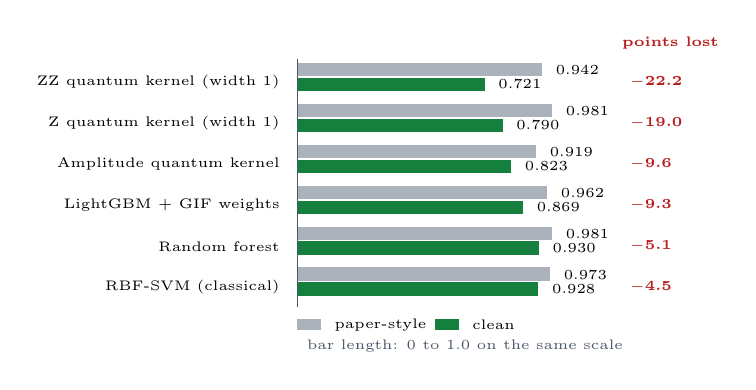
\begin{tikzpicture}[font=\tiny,x=1cm,y=1cm]
        \pgfmathsetmacro{\sc}{3.3}
        \foreach \lab/\lk/\cl/\gp [count=\i] in {ZZ quantum kernel (width 1)/0.942/0.721/22.2,Z quantum kernel (width 1)/0.981/0.790/19.0,Amplitude quantum kernel/0.919/0.823/9.6,LightGBM + GIF weights/0.962/0.869/9.3,Random forest/0.981/0.930/5.1,RBF-SVM (classical)/0.973/0.928/4.5}{
          \pgfmathsetmacro{\y}{-0.52*\i}
          \node[anchor=east,font=\tiny] at (2.55,\y-0.08){\lab};
          \fill[qslate!45](2.65,\y)rectangle({2.65+\sc*\lk},\y+0.17);
          \fill[qgreen](2.65,\y-0.19)rectangle({2.65+\sc*\cl},\y-0.02);
          \node[anchor=west,font=\tiny] at ({2.7+\sc*\lk},\y+0.08){\lk};
          \node[anchor=west,font=\tiny] at ({2.7+\sc*\cl},\y-0.1){\cl};
          \node[anchor=west,font=\tiny\bfseries,text=qcrimson] at (6.75,\y-0.08){$-$\gp};
        }
        \draw[qslate](2.65,-0.3)--(2.65,-3.45);
        \node[font=\tiny\bfseries,anchor=west,text=qcrimson] at (6.65,-0.1){points lost};
        \fill[qslate!45](2.65,-3.75)rectangle++(0.3,0.14);\node[anchor=west] at (3.0,-3.68){paper-style};
        \fill[qgreen](4.4,-3.75)rectangle++(0.3,0.14);\node[anchor=west] at (4.75,-3.68){clean};
        \node[anchor=west,text=qslate] at (2.65,-3.95){bar length: 0 to 1.0 on the same scale};
      \end{tikzpicture}}
  \end{columns}
  \vspace{2pt}
  {\scriptsize\textbf{Takeaway:} Fine-grained quantum models memorize duplicate profiles. When duplicates are blocked, ZZ-QSVM collapses by \bval{22.1\%}.\par}
  \pfoot{ZZ, Z, Amplitude = quantum feature maps. GIF = graph intuitionistic fuzzy sample weighting. RBF-SVM = classical support vector machine. Sylhet = questionnaire ($N=520$). Points lost computed from unrounded report values.}
\end{frame}

% ==============================================================================
% SLIDE 9: Finding 2: No Quantum Advantage
% ==============================================================================
\begin{frame}{Finding 2: No Quantum Advantage Across Any Cohort}
  \begin{columns}[T]
    \column{0.55\textwidth}
      \centering
      {\scriptsize\textbf{Balanced accuracy (0.5 = coin flip, 1.0 = perfect)}}\\[2pt]
      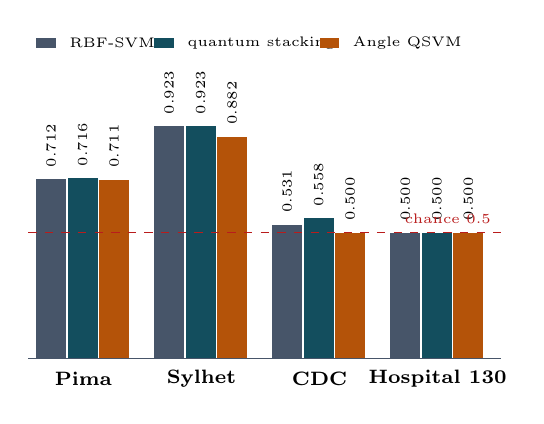
\begin{tikzpicture}[font=\tiny,x=1cm,y=1cm]
        \pgfmathsetmacro{\hs}{3.2}
        \foreach \g/\nm/\a/\b/\c in {0/Pima/0.712/0.716/0.711,1/Sylhet/0.923/0.923/0.882,2/CDC/0.531/0.558/0.500,3/Hospital 130/0.500/0.500/0.500}{
          \pgfmathsetmacro{\x}{1.5*\g}
          \fill[qslate](\x,0)rectangle++(0.38,{\hs*\a});
          \fill[qteal]({\x+0.4},0)rectangle++(0.38,{\hs*\b});
          \fill[qamber]({\x+0.8},0)rectangle++(0.38,{\hs*\c});
          \node[anchor=south,rotate=90,anchor=west] at ({\x+0.19},{\hs*\a+0.03}){\a};
          \node[anchor=south,rotate=90,anchor=west] at ({\x+0.59},{\hs*\b+0.03}){\b};
          \node[anchor=south,rotate=90,anchor=west] at ({\x+0.99},{\hs*\c+0.03}){\c};
          \node[font=\scriptsize\bfseries] at ({\x+0.6},-0.25){\nm};
        }
        \draw[qslate](-0.1,0)--(5.9,0);
        \draw[qcrimson,dashed]({-0.1},{\hs*0.5})--(5.9,{\hs*0.5})node[anchor=south east,text=qcrimson]{chance 0.5};
        \fill[qslate](0,3.95)rectangle++(0.25,0.12);\node[anchor=west] at (0.3,4.01){RBF-SVM};
        \fill[qteal](1.5,3.95)rectangle++(0.25,0.12);\node[anchor=west] at (1.8,4.01){quantum stacking};
        \fill[qamber](3.6,3.95)rectangle++(0.25,0.12);\node[anchor=west] at (3.9,4.01){Angle QSVM};
      \end{tikzpicture}
    \column{0.43\textwidth}
      \centering
      {\scriptsize\textbf{Models vs Classical RBF-SVM (36 tests each)}}\\[2pt]
      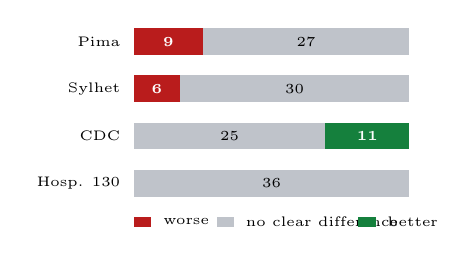
\begin{tikzpicture}[font=\tiny,x=1cm,y=1cm]
        \pgfmathsetmacro{\cs}{3.5/36}
        \foreach \nm/\w/\n/\b [count=\i] in {Pima/9/27/0,Sylhet/6/30/0,CDC/0/25/11,Hosp. 130/0/36/0}{
          \pgfmathsetmacro{\y}{-0.6*\i+0.4}
          \node[anchor=east] at (1.0,\y){\nm};
          \pgfmathsetmacro{\xa}{1.05+\cs*\w}
          \pgfmathsetmacro{\xb}{1.05+\cs*(\w+\n)}
          \pgfmathsetmacro{\xc}{1.05+\cs*(\w+\n+\b)}
          \ifnum\w>0 \fill[qcrimson](1.05,\y-0.17)rectangle(\xa,\y+0.17);\node[text=white,font=\tiny\bfseries] at ({(1.05+\xa)/2},\y){\w};\fi
          \fill[qslate!35](\xa,\y-0.17)rectangle(\xb,\y+0.17);\node[font=\tiny] at ({(\xa+\xb)/2},\y){\n};
          \ifnum\b>0 \fill[qgreen](\xb,\y-0.17)rectangle(\xc,\y+0.17);\node[text=white,font=\tiny\bfseries] at ({(\xb+\xc)/2},\y){\b};\fi
        }
        \fill[qcrimson](1.05,-2.55)rectangle++(0.22,0.12);\node[anchor=west] at (1.3,-2.49){worse};
        \fill[qslate!35](2.1,-2.55)rectangle++(0.22,0.12);\node[anchor=west] at (2.35,-2.49){no clear difference};
        \fill[qgreen](3.9,-2.55)rectangle++(0.22,0.12);\node[anchor=west] at (4.15,-2.49){better};
      \end{tikzpicture}\\[2pt]
      {\tiny CDC ``better'' comes from class weighting or a tuned cut-off, not quantum encodings. Pima, Sylhet, Hospital 130: zero quantum models beat classical RBF-SVM.}
  \end{columns}
  \vspace{2pt}
  {\scriptsize Quantum models were exact statevector simulations (up to 8 qubits), representing their theoretical best.\par}
  \pfoot{RBF-SVM = radial basis function support vector machine (classical). QSVM = quantum support vector machine. Stacking = meta-learner combining multiple model predictions. CDC = US Centers for Disease Control survey. Hosp. 130 = inpatient records. Tests = Nadeau-Bengio corrected resampled $t$-test with Holm step-down.}
\end{frame}

% ==============================================================================
% SLIDE 10: Finding 3: Entangled Kernels Need Tuning
% ==============================================================================
\begin{frame}{Finding 3: Entangled Quantum Kernels Need Careful Tuning}
  \begin{columns}[T]
    \column{0.48\textwidth}
      \centering
      {\scriptsize\textbf{The Problem: Wild Phase Rotations}}\\[3pt]
      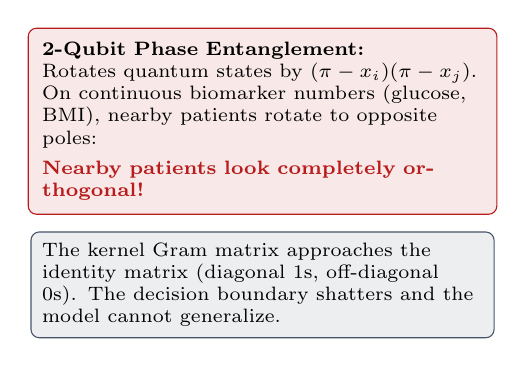
\begin{tikzpicture}[font=\scriptsize]
        \node[pAbx=qcrimson,text width=5.6cm,inner sep=5pt](m){%
          \textbf{2-Qubit Phase Entanglement:}\\
          Rotates quantum states by $(\pi - x_i)(\pi - x_j)$.\\
          On continuous biomarker numbers (glucose, BMI), nearby patients rotate to opposite poles:
          \\[3pt]
          \textcolor{qcrimson}{\textbf{Nearby patients look completely orthogonal!}}
        };
        \node[pAbx=qslate,text width=5.6cm,inner sep=4pt,below=6pt of m]{%
          The kernel Gram matrix approaches the identity matrix (diagonal 1s, off-diagonal 0s). The decision boundary shatters and the model cannot generalize.
        };
      \end{tikzpicture}
    \column{0.50\textwidth}
      \centering
      {\scriptsize\textbf{Default Width vs Tuned Width (Balanced Acc)}}\\[3pt]
      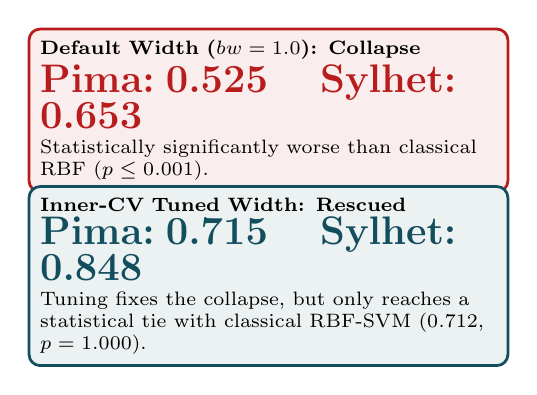
\begin{tikzpicture}[x=1cm,y=1cm]
        \node[pAcard=qcrimson,text width=5.8cm,minimum height=1.7cm] at (0,0){%
          \textbf{Default Width ($bw=1.0$): Collapse}\\[1pt]
          \textcolor{qcrimson}{\pAbig Pima: 0.525 \quad Sylhet: 0.653}\\[1pt]
          Statistically significantly worse than classical RBF ($p \le 0.001$).
        };
        \node[pAcard=qteal,text width=5.8cm,minimum height=1.7cm] at (0,-2.0){%
          \textbf{Inner-CV Tuned Width: Rescued}\\[1pt]
          \textcolor{qteal}{\pAbig Pima: 0.715 \quad Sylhet: 0.848}\\[1pt]
          Tuning fixes the collapse, but only reaches a statistical tie with classical RBF-SVM ($0.712$, $p=1.000$).
        };
      \end{tikzpicture}
  \end{columns}
  \vspace{2pt}
  {\scriptsize\textbf{Takeaway:} Entanglement provides no inductive bias advantage on clinical tables. Untuned, it fails; tuned, it only matches classical tools.\par}
  \pfoot{ZZ = quantum feature map with two-qubit entangling gates ($U_{\text{ZZ}}$). $bw$ = bandwidth scaling factor. Inner-CV = hyperparameter optimization restricted strictly to training folds. RBF-SVM = classical support vector machine. Pima, Sylhet = diabetes cohorts.}
\end{frame}

% ==============================================================================
% SLIDE 11: Finding 4: Uneven Data Blinds Quantum Models
% ==============================================================================
\begin{frame}{Finding 4: Uneven Class Prevalence Blinds Quantum Models}
  \begin{columns}[T]
    \column{0.48\textwidth}
      \centering
      {\scriptsize\textbf{Natural Low Prevalence in Real Life}}\\[3pt]
      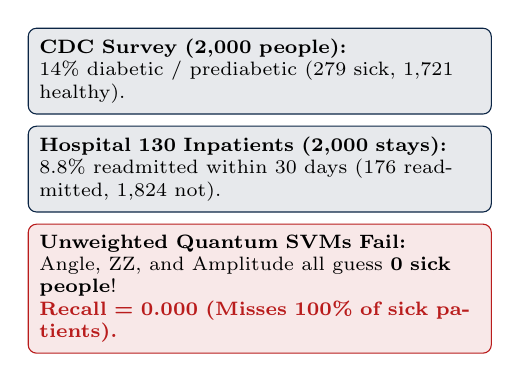
\begin{tikzpicture}[font=\scriptsize]
        \node[pAbx=qnavy,text width=5.6cm,inner sep=4pt](c1){%
          \textbf{CDC Survey (2,000 people):}\\
          14\% diabetic / prediabetic (279 sick, 1,721 healthy).
        };
        \node[pAbx=qnavy,text width=5.6cm,inner sep=4pt,below=4pt of c1](c2){%
          \textbf{Hospital 130 Inpatients (2,000 stays):}\\
          8.8\% readmitted within 30 days (176 readmitted, 1,824 not).
        };
        \node[pAbx=qcrimson,text width=5.6cm,inner sep=4pt,below=4pt of c2](c3){%
          \textbf{Unweighted Quantum SVMs Fail:}\\
          Angle, ZZ, and Amplitude all guess \textbf{0 sick people}!\\
          \textcolor{qcrimson}{\textbf{Recall = 0.000 (Misses 100\% of sick patients).}}
        };
      \end{tikzpicture}
    \column{0.50\textwidth}
      \centering
      {\scriptsize\textbf{CDC Benchmark: Plain Accuracy Masks Failure}}\\[3pt]
      \renewcommand{\arraystretch}{1.12}
      \resizebox{\linewidth}{!}{%
      \begin{tabular}{lcccc}
        \toprule
        \textbf{Model on CDC} & \textbf{Accuracy} & \textbf{Bal.\ Acc} & \textbf{Recall} & \textbf{Verdict} \\
        \midrule
        Always say ``healthy'' & 86.0\% & 0.500 & \bval{0.000} & Useless \\
        Angle QSVM (quantum)   & 86.0\% & 0.500 & \bval{0.000} & \bval{Misses all} \\
        Amplitude QSVM         & 86.0\% & 0.500 & \bval{0.000} & \bval{Misses all} \\
        Plain Classical RBF    & 86.2\% & 0.531 & 0.071 & Poor \\
        \midrule
        Balanced RBF (Kiran)   & 71.6\% & \gval{0.727} & \gval{0.786} & \gval{Finds 79\%} \\
        DiaBeats Tuned RF      & 70.1\% & \gval{0.721} & \gval{0.748} & \gval{Finds 75\%} \\
        \bottomrule
      \end{tabular}}
      \vspace{4pt}
      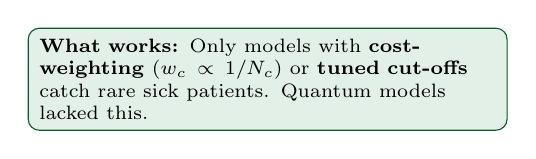
\begin{tikzpicture}[font=\scriptsize]
        \node[draw=qgreen!70!black,fill=qgreen!12,rounded corners,text width=5.8cm,inner sep=4pt]{%
          \textbf{What works:} Only models with \textbf{cost-weighting} ($w_c \propto 1/N_c$) or \textbf{tuned cut-offs} catch rare sick patients. Quantum models lacked this.
        };
      \end{tikzpicture}
  \end{columns}
  \pfoot{CDC = US Centers for Disease Control survey. Recall = sensitivity (share of sick people found). Balanced accuracy = average of recall and specificity. QSVM = quantum support vector machine. RF = random forest. High accuracy (86\%) simply reflects the majority baseline.}
\end{frame}

% ==============================================================================
% SLIDE 12: Finding 5: Amplitude Encoding Erases Biological Scale
% ==============================================================================
\begin{frame}{Finding 5: Amplitude Encoding Erases Biological Scale}
  \begin{columns}[T]
    \column{0.50\textwidth}
      \centering
      {\scriptsize\textbf{The Math: Mandatory Length Normalization}}\\[3pt]
      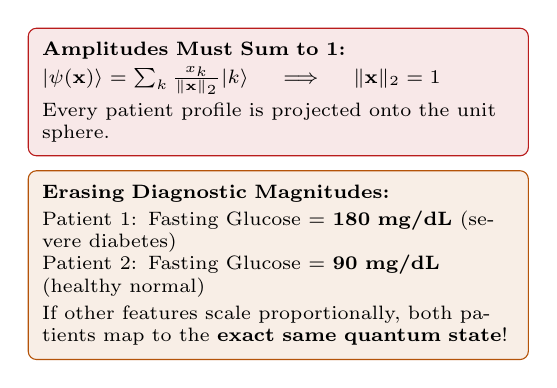
\begin{tikzpicture}[font=\scriptsize]
        \node[pAbx=qcrimson,text width=6.0cm,inner sep=5pt](a){%
          \textbf{Amplitudes Must Sum to 1:}\\[2pt]
          $|\psi(\mathbf{x})\rangle = \sum_{k} \frac{x_k}{\|\mathbf{x}\|_2} |k\rangle \quad \implies \quad \|\mathbf{x}\|_2 = 1$\\[2pt]
          Every patient profile is projected onto the unit sphere.
        };
        \node[pAbx=qamber,text width=6.0cm,inner sep=5pt,below=5pt of a](b){%
          \textbf{Erasing Diagnostic Magnitudes:}\\[2pt]
          Patient 1: Fasting Glucose = \textbf{180 mg/dL} (severe diabetes)\\
          Patient 2: Fasting Glucose = \textbf{90 mg/dL} (healthy normal)\\[2pt]
          If other features scale proportionally, both patients map to the \textbf{exact same quantum state}!
        };
      \end{tikzpicture}
    \column{0.48\textwidth}
      \centering
      {\scriptsize\textbf{Empirical Impact Across Cohorts}}\\[3pt]
      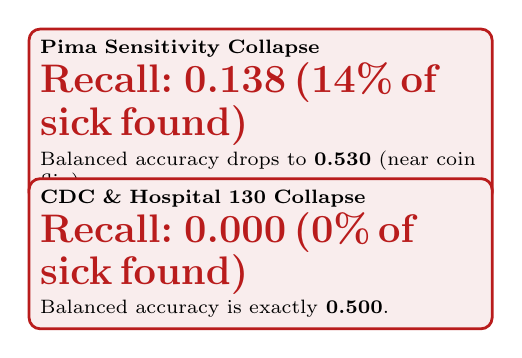
\begin{tikzpicture}[font=\scriptsize,x=1cm,y=1cm]
        \node[pAcard=qcrimson,text width=5.6cm,minimum height=1.6cm] at (0,0){%
          \textbf{Pima Sensitivity Collapse}\\[1pt]
          \textcolor{qcrimson}{\pAbig Recall: 0.138 (14\% of sick found)}\\[1pt]
          Balanced accuracy drops to \textbf{0.530} (near coin flip).
        };
        \node[pAcard=qcrimson,text width=5.6cm,minimum height=1.6cm] at (0,-1.9){%
          \textbf{CDC \& Hospital 130 Collapse}\\[1pt]
          \textcolor{qcrimson}{\pAbig Recall: 0.000 (0\% of sick found)}\\[1pt]
          Balanced accuracy is exactly \textbf{0.500}.
        };
      \end{tikzpicture}
      \vspace{2pt}
      {\scriptsize\textbf{Angle Encoding is Strictly Better:} Angle maps keep each feature on its own axis without losing scale.\par}
  \end{columns}
  \pfoot{Amplitude encoding = storing data in quantum state probabilities. $L_2$ norm = Euclidean length. Recall = share of sick people found. Angle encoding = rotating qubits by feature angles. Pima, CDC, Hospital 130 = diabetes benchmarks.}
\end{frame}

% ==============================================================================
% SLIDE 13: Young: Made-up rows
% ==============================================================================
\begin{frame}{Method Check: Young et al. (Made-Up Test Rows)}
  \begin{columns}[c]
    \column{0.62\textwidth}
      \centering
      {\footnotesize\textbf{Paper-Style Test (with Made-Up Rows) vs Real Patients Only}}\\[3pt]
      \renewcommand{\arraystretch}{1.18}
      \resizebox{\linewidth}{!}{%
      \begin{tabular}{lcccccc}
        \toprule
        & \multicolumn{3}{c}{\textbf{Paper-Style (with Made-Up Rows)}} & \multicolumn{3}{c}{\textbf{Real Patients Only (Clean)}} \\
        \textbf{Dataset} & \textbf{Accuracy} & \textbf{Bal.\ Acc} & \textbf{Recall} & \textbf{Accuracy} & \textbf{Bal.\ Acc} & \textbf{Recall} \\
        \midrule
        Pima         & 0.897 & 0.767 & 0.971 & 0.675 & 0.725 & 0.885 \\
        Sylhet       & 0.996 & 0.987 & 0.998 & 0.985 & 0.983 & 0.992 \\
        CDC Survey   & 0.957 & 0.951 & 0.963 & \bval{0.851} & \bval{0.622} & \bval{0.304} \\
        Hospital 130 & 0.972 & 0.977 & 0.967 & \bval{0.902} & \bval{0.506} & \bval{0.026} \\
        \bottomrule
      \end{tabular}}
      \vspace{4pt}
      {\tiny Numbers are 5-fold CV averages (seed 42) from \texttt{02\_young.csv}. Single run without significance testing.}

    \column{0.36\textwidth}
      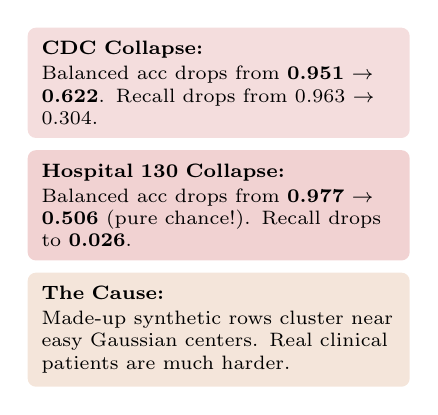
\begin{tikzpicture}[font=\scriptsize,c/.style={draw=none,rounded corners=3pt,text width=4.5cm,inner sep=5pt,align=left}]
        \node[c,fill=qcrimson!15](a){%
          \textbf{CDC Collapse:}\\[1pt]
          Balanced acc drops from \textbf{0.951 $\to$ 0.622}. Recall drops from 0.963 $\to$ 0.304.
        };
        \node[c,fill=qcrimson!20,below=4pt of a](b){%
          \textbf{Hospital 130 Collapse:}\\[1pt]
          Balanced acc drops from \textbf{0.977 $\to$ 0.506} (pure chance!). Recall drops to \textbf{0.026}.
        };
        \node[c,fill=qamber!15,below=4pt of b](d){%
          \textbf{The Cause:}\\[1pt]
          Made-up synthetic rows cluster near easy Gaussian centers. Real clinical patients are much harder.
        };
      \end{tikzpicture}
  \end{columns}
  \pfoot{Young et al. = QISICGM model with Gaussian Mixture Model (GMM) synthetic data augmentation. Made-up rows = computer-generated minority samples. Clean = synthetic samples restricted to training folds; test fold evaluates real patients only. CDC, Hosp 130 = imbalanced cohorts.}
\end{frame}

% ==============================================================================
% SLIDE 14: Zhang: Label Noise
% ==============================================================================
\begin{frame}{Method Check: Zhang et al. (Noisy Training Labels)}
  \begin{columns}[c]
    \column{0.62\textwidth}
      \centering
      {\footnotesize\textbf{Plain LightGBM vs LightGBM + GIF Sample Weights}}\\[3pt]
      \renewcommand{\arraystretch}{1.15}
      \resizebox{\linewidth}{!}{%
      \begin{tabular}{llcccccc}
        \toprule
        & & \multicolumn{3}{c}{\textbf{Balanced Accuracy}} & \multicolumn{3}{c}{\textbf{Recall (Sick Found)}} \\
        \textbf{Dataset} & \textbf{Model} & \textbf{0\% Noise} & \textbf{20\%} & \textbf{40\%} & \textbf{0\% Noise} & \textbf{20\%} & \textbf{40\%} \\
        \midrule
        Pima   & Plain     & 0.712 & 0.678 & 0.545 & 0.582 & 0.574 & 0.495 \\
        Pima   & + GIF     & \gval{0.732} & \gval{0.712} & \gval{0.638} & \gval{0.612} & \gval{0.600} & \gval{0.574} \\
        \midrule
        Sylhet & Plain     & 0.972 & 0.896 & 0.653 & 0.969 & 0.913 & 0.681 \\
        Sylhet & + GIF     & 0.964 & 0.891 & \gval{0.735} & 0.953 & 0.881 & \gval{0.716} \\
        \midrule
        CDC    & Plain     & 0.583 & 0.587 & 0.547 & 0.201 & 0.229 & 0.315 \\
        CDC    & + GIF     & 0.591 & 0.565 & 0.577 & 0.222 & 0.179 & 0.304 \\
        \midrule
        Hosp 130 & Plain   & 0.502 & 0.500 & 0.505 & 0.006 & 0.011 & 0.211 \\
        Hosp 130 & + GIF   & 0.500 & 0.508 & 0.536 & 0.011 & 0.051 & 0.250 \\
        \bottomrule
      \end{tabular}}
      \vspace{4pt}
      {\tiny Numbers are fold averages from \texttt{04\_zhang.csv}. Flipped labels applied to training folds only.}

    \column{0.36\textwidth}
      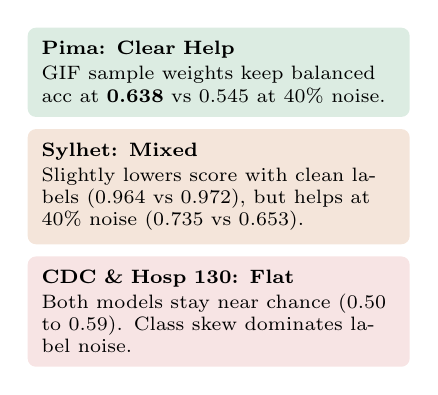
\begin{tikzpicture}[font=\scriptsize,c/.style={draw=none,rounded corners=3pt,text width=4.5cm,inner sep=5pt,align=left}]
        \node[c,fill=qgreen!15](a){%
          \textbf{Pima: Clear Help}\\[1pt]
          GIF sample weights keep balanced acc at \textbf{0.638} vs 0.545 at 40\% noise.
        };
        \node[c,fill=qamber!15,below=4pt of a](b){%
          \textbf{Sylhet: Mixed}\\[1pt]
          Slightly lowers score with clean labels (0.964 vs 0.972), but helps at 40\% noise (0.735 vs 0.653).
        };
        \node[c,fill=qcrimson!12,below=4pt of b](d){%
          \textbf{CDC \& Hosp 130: Flat}\\[1pt]
          Both models stay near chance (0.50 to 0.59). Class skew dominates label noise.
        };
      \end{tikzpicture}
  \end{columns}
  \pfoot{Zhang et al. = DeSCN model with Graph Intuitionistic Fuzzy (GIF) sample weighting. Noise = randomly flipped labels in training. LightGBM = classical gradient boosted decision trees. Balanced accuracy = average of recall and specificity.}
\end{frame}

% ==============================================================================
% SLIDE 15: Visual Map: Heatmap
% ==============================================================================
\begin{frame}{Visual Synthesis: Balanced Accuracy Across All Methods}
  \begin{columns}[c]
    \column{0.56\textwidth}
      \centering
      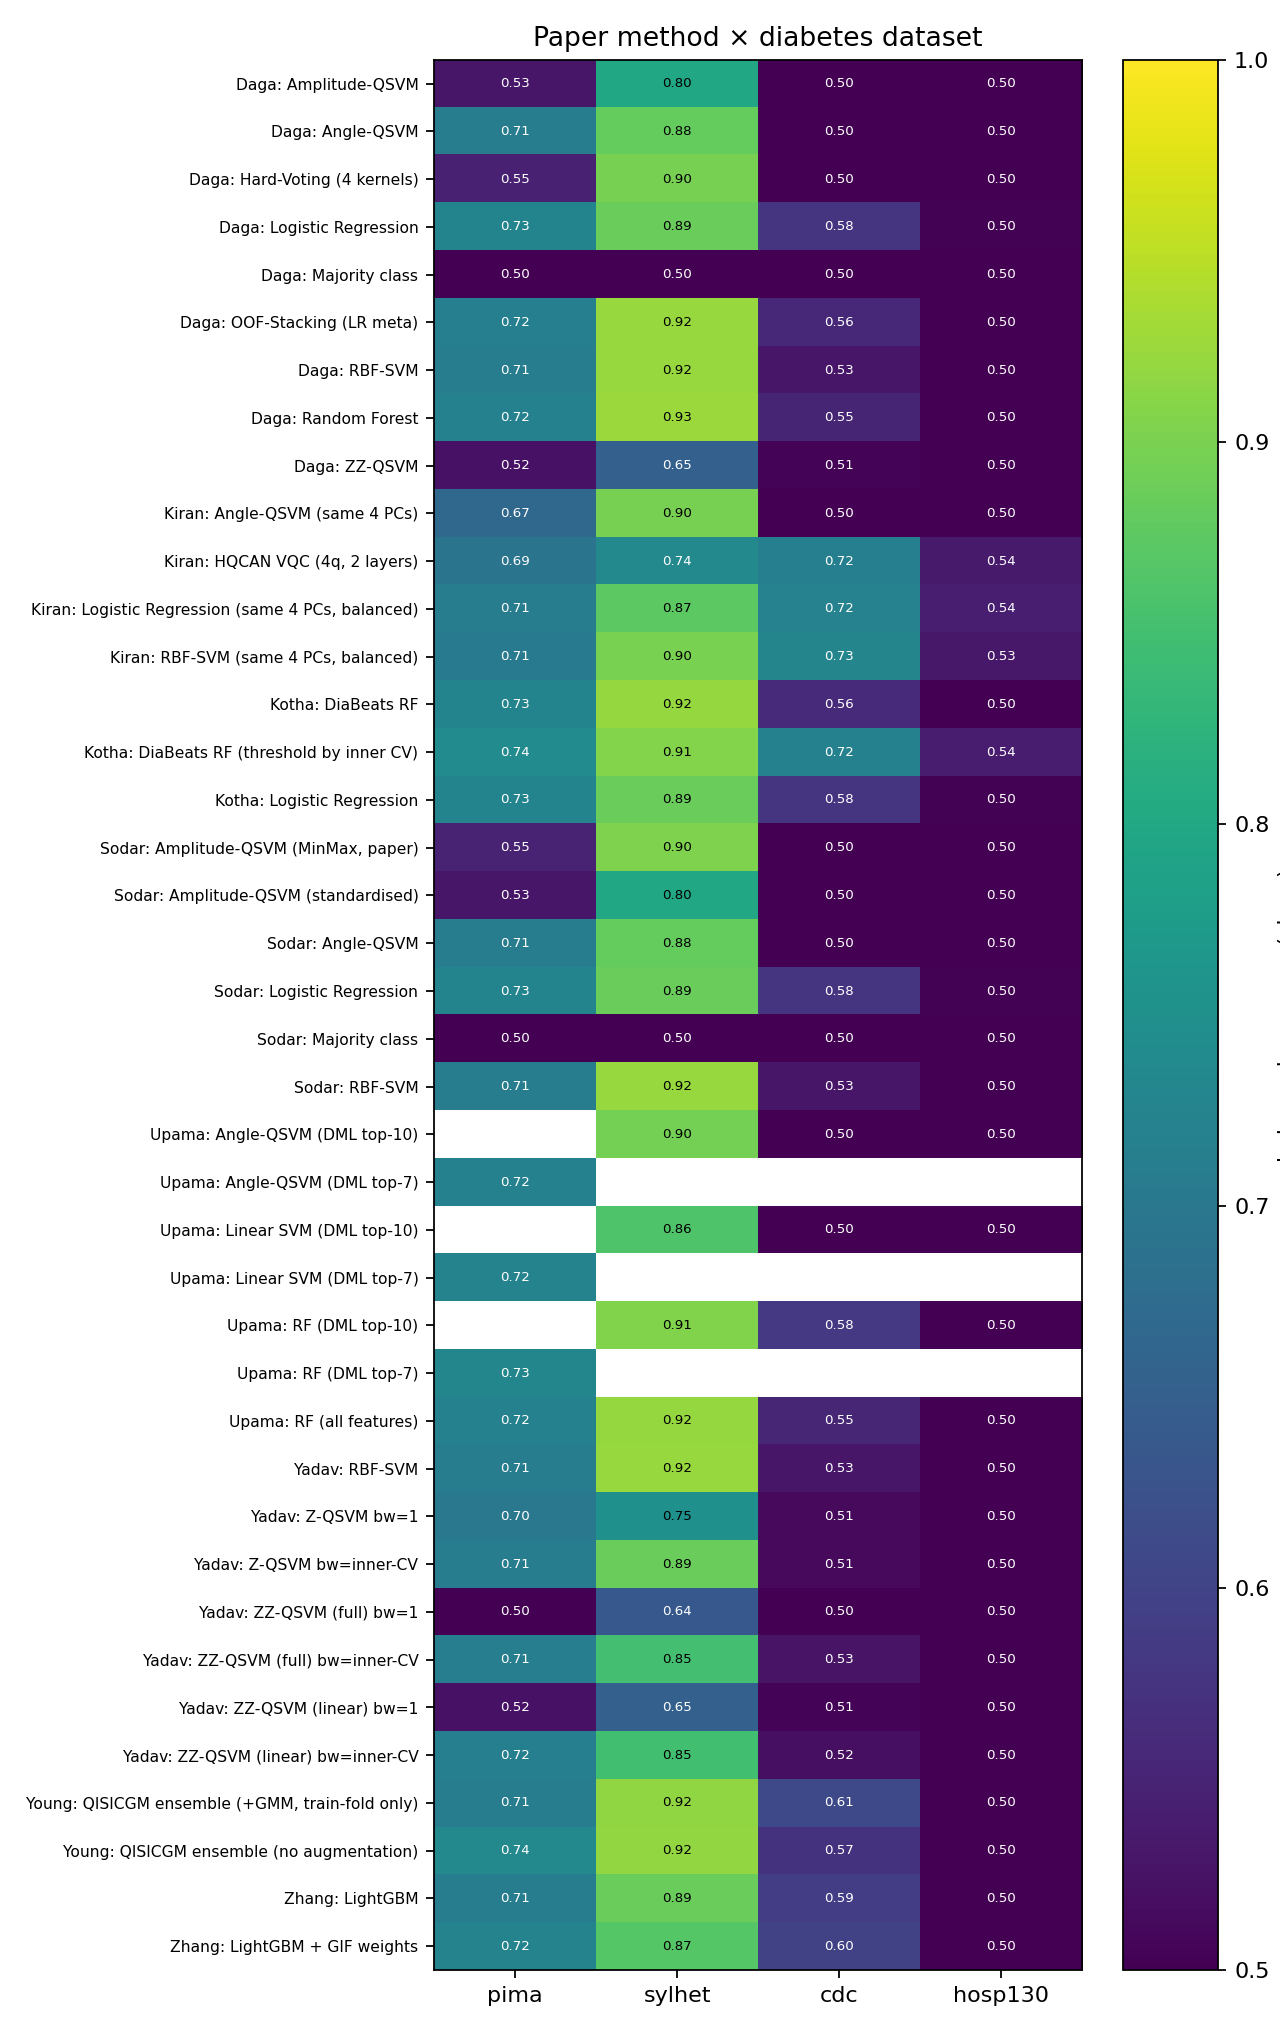
\includegraphics[width=\linewidth,height=0.74\textheight,keepaspectratio]{09_heatmap_balanced_accuracy.png}

    \column{0.41\textwidth}
      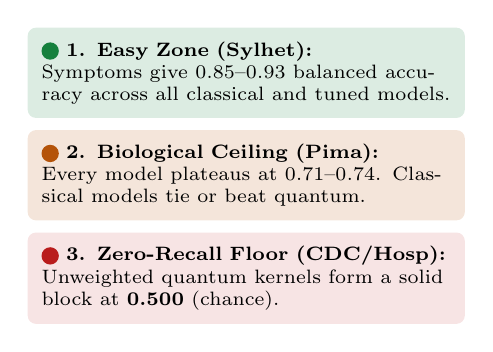
\begin{tikzpicture}[font=\scriptsize,c/.style={draw=none,rounded corners=3pt,text width=5.2cm,inner sep=5pt,align=left}]
        \node[c,fill=qgreen!15](a){%
          \tlC{qgreen}\ \textbf{1. Easy Zone (Sylhet):}\\
          Symptoms give $0.85\text{--}0.93$ balanced accuracy across all classical and tuned models.
        };
        \node[c,fill=qamber!15,below=4pt of a](b){%
          \tlC{qamber}\ \textbf{2. Biological Ceiling (Pima):}\\
          Every model plateaus at $0.71\text{--}0.74$. Classical models tie or beat quantum.
        };
        \node[c,fill=qcrimson!12,below=4pt of b](d){%
          \tlC{qcrimson}\ \textbf{3. Zero-Recall Floor (CDC/Hosp):}\\
          Unweighted quantum kernels form a solid block at \textbf{0.500} (chance).
        };
      \end{tikzpicture}
      \vspace{4pt}
      {\tiny Heatmap generated directly from notebook execution results (\texttt{09\_summary.ipynb}).}
  \end{columns}
  \pfoot{Balanced accuracy scale: yellow/green = high ($>0.80$), purple/blue = chance ($0.50$). Pima, Sylhet, CDC, Hospital 130 = four audited diabetes cohorts. All evaluations clean, leakage-free 15 folds.}
\end{frame}

% ==============================================================================
% SLIDE 16: Scoreboard: Who Gets It Right?
% ==============================================================================
\begin{frame}{Scoreboard: Who Gets It Right?}
  \begin{columns}[c]
    \column{0.60\textwidth}
      \centering
      {\footnotesize\textbf{Balanced accuracy} (0.5 = coin flip, 1.0 = perfect)}\\[2pt]
      \renewcommand{\arraystretch}{1.10}
      \resizebox{\linewidth}{!}{%
      \begin{tabular}{@{}l|cccc@{}}
        \toprule
        \textbf{Method} & \textbf{Pima} & \textbf{Sylhet} & \textbf{CDC} & \textbf{Hosp 130}\\
        \midrule
        RBF-SVM (classical)        & \cbaC{0.712} & \cbaC{0.923} & \cbaC{0.531} & \cbaC{0.500}\\
        Random forest              & \cbaC{0.720} & \cbaC{0.925} & \cbaC{0.551} & \cbaC{0.500}\\
        Random forest, tuned cut-off & \cbaC{0.741} & \cbaC{0.907} & \cbaC{0.721} & \cbaC{0.538}\\
        Angle QSVM                 & \cbaC{0.711} & \cbaC{0.882} & \cbaC{0.500} & \cbaC{0.500}\\
        ZZ QSVM (default)          & \cbaC{0.525} & \cbaC{0.653} & \cbaC{0.506} & \cbaC{0.500}\\
        ZZ QSVM (tuned width)      & \cbaC{0.715} & \cbaC{0.848} & \cbaC{0.520} & \cbaC{0.500}\\
        Amplitude QSVM             & \cbaC{0.530} & \cbaC{0.798} & \cbaC{0.500} & \cbaC{0.500}\\
        Stacking of 4 kernels      & \cbaC{0.716} & \cbaC{0.923} & \cbaC{0.558} & \cbaC{0.500}\\
        VQC (4 qubits)             & \cbaC{0.693} & \cbaC{0.736} & \cbaC{0.715} & \cbaC{0.536}\\
        \midrule
        Always guess biggest group & \cbaC{0.500} & \cbaC{0.500} & \cbaC{0.500} & \cbaC{0.500}\\
        \bottomrule
      \end{tabular}}\\[3pt]
      {\tiny colour key:\ \colorbox{qcrimson!30}{\,below 0.55\,}\ \colorbox{qamber!35}{\,0.55--0.65\,}\ \colorbox{qamber!12}{\,0.65--0.80\,}\ \colorbox{qgreen!20}{\,0.80--0.88\,}\ \colorbox{qgreen!38}{\,0.88 and up\,}}

    \column{0.37\textwidth}
      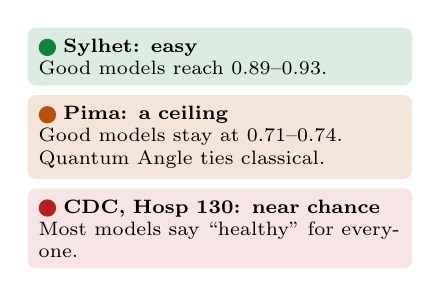
\begin{tikzpicture}[font=\scriptsize,c/.style={draw=none,rounded corners=3pt,text width=4.6cm,inner sep=4pt,align=left}]
        \node[c,fill=qgreen!15](a){\tlC{qgreen} \textbf{Sylhet: easy}\\ Good models reach 0.89--0.93.};
        \node[c,fill=qamber!15,below=3pt of a](b){\tlC{qamber} \textbf{Pima: a ceiling}\\ Good models stay at 0.71--0.74. Quantum Angle ties classical.};
        \node[c,fill=qcrimson!12,below=3pt of b](d){\tlC{qcrimson} \textbf{CDC, Hosp 130: near chance}\\ Most models say ``healthy'' for everyone.};
      \end{tikzpicture}
  \end{columns}
  \pfoot{RBF-SVM = classical support vector machine; QSVM = quantum SVM (simulated); Angle, ZZ, Amplitude = quantum encodings; VQC = variational quantum classifier; CDC = CDC health survey; Hosp 130 = hospital data; Pima, Sylhet = diabetes cohorts. Clean 15-fold means.}
\end{frame}

% ==============================================================================
% SLIDE 17: The Full Numbers
% ==============================================================================
\begin{frame}{The Full Numbers: Balanced Accuracy, Recall, Specificity}
  \centering
  \resizebox{\textwidth}{!}{%
  \begin{tabular}{l|ccc|ccc|ccc|ccc}
    \toprule
    & \multicolumn{3}{c|}{\textbf{Pima} (768 rows)} & \multicolumn{3}{c|}{\textbf{Sylhet} (520)} & \multicolumn{3}{c|}{\textbf{CDC} (2,000)} & \multicolumn{3}{c}{\textbf{Hosp 130} (2,000)}\\
    \textbf{Method} & BA & Rec & Spec & BA & Rec & Spec & BA & Rec & Spec & BA & Rec & Spec\\
    \midrule
    RBF-SVM            & \cbaC{0.712} & 0.556 & 0.869 & \cbaC{0.923} & 0.940 & 0.905 & \cbaC{0.531} & 0.071 & 0.990 & \cbaC{0.500} & 0.000 & 1.000\\
    Logistic regression& \cbaC{0.726} & 0.571 & 0.881 & \cbaC{0.886} & 0.914 & 0.857 & \cbaC{0.577} & 0.180 & 0.974 & \cbaC{0.503} & 0.009 & 0.996\\
    Random forest      & \cbaC{0.720} & 0.586 & 0.853 & \cbaC{0.925} & 0.943 & 0.908 & \cbaC{0.551} & 0.120 & 0.983 & \cbaC{0.500} & 0.000 & 0.999\\
    RF, tuned cut-off  & \cbaC{0.741} & 0.760 & 0.722 & \cbaC{0.907} & 0.910 & 0.904 & \cbaC{0.721} & 0.748 & 0.694 & \cbaC{0.538} & 0.437 & 0.640\\
    \midrule
    Angle QSVM         & \cbaC{0.711} & 0.552 & 0.870 & \cbaC{0.882} & 0.918 & 0.846 & \cbaC{0.500} & 0.000 & 1.000 & \cbaC{0.500} & 0.000 & 1.000\\
    ZZ QSVM (default)  & \cbaC{0.525} & 0.082 & 0.967 & \cbaC{0.653} & 0.985 & 0.322 & \cbaC{0.506} & 0.014 & 0.998 & \cbaC{0.500} & 0.000 & 1.000\\
    ZZ QSVM (tuned)    & \cbaC{0.715} & 0.556 & 0.874 & \cbaC{0.848} & 0.878 & 0.817 & \cbaC{0.520} & 0.049 & 0.992 & \cbaC{0.500} & 0.000 & 1.000\\
    Amplitude QSVM     & \cbaC{0.530} & 0.138 & 0.921 & \cbaC{0.798} & 0.903 & 0.693 & \cbaC{0.500} & 0.000 & 1.000 & \cbaC{0.500} & 0.000 & 1.000\\
    Stacking (OOF)     & \cbaC{0.716} & 0.567 & 0.865 & \cbaC{0.923} & 0.929 & 0.917 & \cbaC{0.558} & 0.133 & 0.982 & \cbaC{0.500} & 0.000 & 1.000\\
    VQC (4 qubits)     & \cbaC{0.693} & 0.691 & 0.695 & \cbaC{0.736} & 0.760 & 0.712 & \cbaC{0.715} & 0.714 & 0.716 & \cbaC{0.536} & 0.497 & 0.576\\
    \midrule
    Guess biggest group& \cbaC{0.500} & 0.000 & 1.000 & \cbaC{0.500} & 1.000 & 0.000 & \cbaC{0.500} & 0.000 & 1.000 & \cbaC{0.500} & 0.000 & 1.000\\
    \bottomrule
  \end{tabular}}
  \vspace{3pt}

  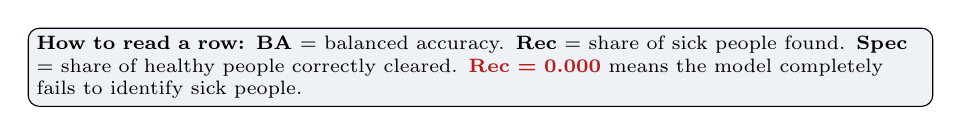
\begin{tikzpicture}[font=\scriptsize]
    \node[draw,rounded corners,fill=qcard,text width=0.93\textwidth,inner sep=3pt,align=left]{%
      \textbf{How to read a row:} \textbf{BA} = balanced accuracy. \textbf{Rec} = share of sick people found. \textbf{Spec} = share of healthy people correctly cleared. \textcolor{qcrimson}{\textbf{Rec = 0.000}} means the model completely fails to identify sick people.};
  \end{tikzpicture}
  \pfoot{BA = balanced accuracy (average of Rec and Spec); Rec = recall (sensitivity); Spec = specificity; RF = random forest (tuned cut-off = inner-CV threshold); OOF = out-of-fold; QSVM = quantum support vector machine; VQC = variational quantum classifier; RBF = radial basis function; SVM = support vector machine. Mean of 15 folds.}
\end{frame}

% ==============================================================================
% SLIDE 18: Is Any Model Really Better Than Classical?
% ==============================================================================
\begin{frame}{Is Any Model Really Better Than the Classical One?}
  \begin{columns}[T]
    \column{0.47\textwidth}
      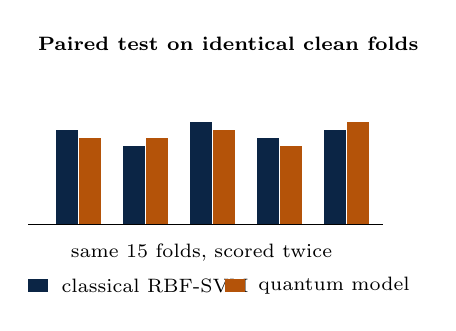
\begin{tikzpicture}[font=\scriptsize,x=1cm,y=1cm]
        \node[anchor=west] at (0,2.3) {\textbf{Paired test on identical clean folds}};
        \foreach \i/\a/\b in {0/1.2/1.1,1/1.0/1.1,2/1.3/1.2,3/1.1/1.0,4/1.2/1.3}{
          \fill[qnavy] (0.35+0.85*\i,0) rectangle ++(0.28,\a);
          \fill[qamber] (0.65+0.85*\i,0) rectangle ++(0.28,\b);
        }
        \draw (0,0)--(4.5,0);
        \node at (2.2,-0.35){same 15 folds, scored twice};
        \fill[qnavy] (0,-0.85) rectangle ++(0.25,0.16); \node[anchor=west] at (0.3,-0.77){classical RBF-SVM};
        \fill[qamber] (2.5,-0.85) rectangle ++(0.25,0.16); \node[anchor=west] at (2.8,-0.77){quantum model};
      \end{tikzpicture}\\[2pt]
      \scriptsize Both models scored on identical splits. We test whether differences exceed statistical noise.\\[3pt]
      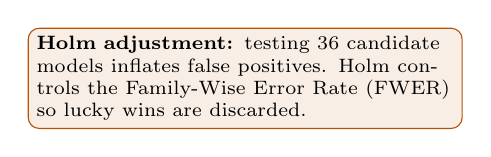
\begin{tikzpicture}[font=\scriptsize]
        \node[draw=qamber,rounded corners,fill=qamber!10,text width=5.3cm,inner sep=3pt]{%
          \textbf{Holm adjustment:} testing 36 candidate models inflates false positives. Holm controls the Family-Wise Error Rate (FWER) so lucky wins are discarded.};
      \end{tikzpicture}

    \column{0.51\textwidth}
      {\footnotesize\textbf{Models compared with RBF-SVM} (36 tests per dataset)}\\[3pt]
      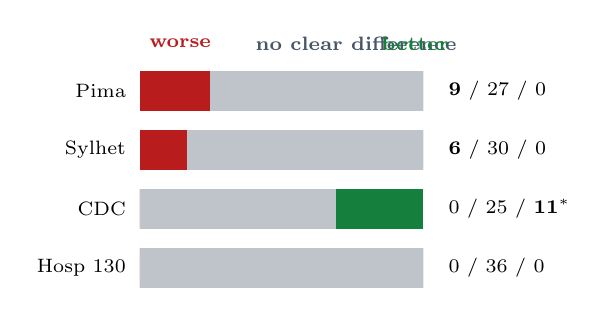
\begin{tikzpicture}[font=\scriptsize,x=0.1cm]
        \foreach \n/\w/\s/\b/\y in {Pima/9/0/27/0, Sylhet/6/0/30/-0.75, CDC/0/11/25/-1.5, {Hosp 130}/0/0/36/-2.25}{
          \node[anchor=east] at (0,\y){\n};
          \pgfmathsetmacro{\xa}{\w}
          \pgfmathsetmacro{\xb}{\w+\b}
          \pgfmathsetmacro{\xc}{\w+\b+\s}
          \fill[qcrimson] (0.5,\y-0.25) rectangle (0.5+\xa,\y+0.25);
          \fill[qslate!35] (0.5+\xa,\y-0.25) rectangle (0.5+\xb,\y+0.25);
          \fill[qgreen] (0.5+\xb,\y-0.25) rectangle (0.5+\xc,\y+0.25);
        }
        \node[anchor=west,text=qcrimson] at (0.5,0.6){\textbf{worse}};
        \node[anchor=west,text=qslate] at (14,0.6){\textbf{no clear difference}};
        \node[anchor=west,text=qgreen] at (30,0.6){\textbf{better}};
        \node[anchor=west] at (38.5,0){\textbf{9} / 27 / 0};
        \node[anchor=west] at (38.5,-0.75){\textbf{6} / 30 / 0};
        \node[anchor=west] at (38.5,-1.5){0 / 25 / \textbf{11}$^*$};
        \node[anchor=west] at (38.5,-2.25){0 / 36 / 0};
      \end{tikzpicture}\\[2pt]
      {\tiny $^*$CDC ``better'' models beat an unweighted RBF-SVM that finds 7\% of sick people. The cause is cost-weighting, not quantum physics.}\\[3pt]
      
\begin{tikzpicture}
        \node[draw=qgreen!60!black,fill=qgreen!15,rounded corners,text width=0.9\textwidth,inner sep=4pt,align=center]{\tlC{qgreen}\ \textbf{Zero quantum models beat classical RBF-SVM on Pima, Sylhet, or Hosp 130.}};
      \end{tikzpicture}
  \end{columns}
  \pfoot{RBF = radial basis function; SVM = support vector machine; ZZ, Amplitude = quantum encodings; CDC = US Centers for Disease Control survey. Test = Nadeau-Bengio corrected resampled $t$-test (accounts for cross-validation fold dependence) on balanced accuracy, Holm-adjusted.}
\end{frame}

% ==============================================================================
% SLIDE 19: Paper Claims vs What We Measured
% ==============================================================================
\begin{frame}{Paper Claims vs What We Measured}
  \centering
  \renewcommand{\arraystretch}{0.84}
  \resizebox{0.97\textwidth}{!}{%
  \begin{tabular}{@{}l p{3.8cm} p{4.5cm} p{5.8cm} c@{}}
    \toprule
    \textbf{Paper} & \textbf{Claimed} & \textbf{We measured} & \textbf{Explanation \& Reconciliation} & \\
    \midrule
    Upama (Sylhet) & 97.1\% accuracy (random forest) & 98.1\% on random split, 91.8\% clean & 269 duplicate questionnaire rows inflate random splits. Grouped CV drops score to 91.8\%. & \tlC{qamber}\\
    Kotha (Pima) & 83.3\% accuracy, AUC 1.00 & 76.0\% accuracy, AUC 0.825 & Claiming AUC 1.00 with 25 errors violates the Mann-Whitney $U$ bound ($\text{AUC} \le 0.9700$). & \tlC{qcrimson}\\
    Kiran (Pima) & 99.7\% accuracy & 67.5\% (paper-style), 69.4\% (clean) & Internal contradiction: paper text reports a 4\% error rate ($96\%$ max). Honest 4-qubit VQC gets 69.4\%. & \tlC{qcrimson}\\
    Daga (Pima) & Stacking 76.6\%; ZZ 75.9\%, Amplitude 76.3\% & Stacking 75.9\% (matches); ZZ 66.3\%, Amplitude 63.8\% & Stacking and Angle match. Original ZZ used PennyLane IQPEmbedding and hard voting with class-weighting. & \tlC{qamber}\\
    Young (all four) & F1 0.8933, AUC 0.8699 & CDC: 0.951 $\to$ 0.622; Hosp: 0.977 $\to$ 0.506 on real patients & Claimed scores rely on made-up GMM rows in test sets. Real clinical patients collapse to chance. & \tlC{qcrimson}\\
    Sodar (Pima) & Amplitude QSVM advantage & Amplitude recall 0.138 (standardized) & Amplitude $L_2$ normalization erases glucose and BMI scale magnitudes. Angle is strictly superior. & \tlC{qamber}\\
    \bottomrule
  \end{tabular}}
  \vspace{3pt}

  {\scriptsize \tlC{qcrimson} refuted / not reproduced \quad \tlC{qamber} reconciled / partially reproduced \quad \tlC{qgreen} fully verified}
  \pfoot{AUC = area under ROC curve; QSVM = quantum SVM; ZZ, Amplitude = quantum encodings; F1 = harmonic mean of precision and recall; CDC = Centers for Disease Control; Hosp = hospital data. Accuracies from report paper-style and clean protocol runs.}
\end{frame}

% ==============================================================================
% SLIDE 20: How This Run Compares With Earlier Work
% ==============================================================================
\begin{frame}{How This Run Compares With Earlier Project Phases}
  \centering
  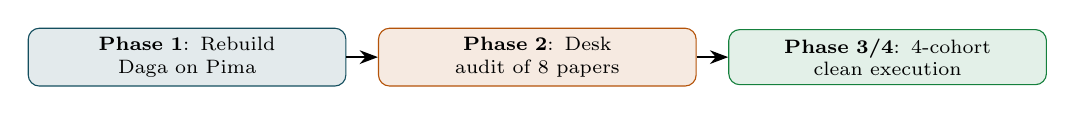
\begin{tikzpicture}[font=\scriptsize,node distance=0.4cm]
    \node[draw=qteal,fill=qteal!12,rounded corners,align=center,text width=3.8cm,minimum height=0.55cm](a){\textbf{Phase 1}: Rebuild Daga on Pima};
    \node[draw=qamber,fill=qamber!12,rounded corners,align=center,text width=3.8cm,minimum height=0.55cm,right=of a](b2){\textbf{Phase 2}: Desk audit of 8 papers};
    \node[draw=qgreen,fill=qgreen!12,rounded corners,align=center,text width=3.8cm,minimum height=0.55cm,right=of b2](c){\textbf{Phase 3/4}: 4-cohort clean execution};
    \draw[-{Stealth},thick](a)--(b2);\draw[-{Stealth},thick](b2)--(c);
  \end{tikzpicture}
  \vspace{1pt}

  \renewcommand{\arraystretch}{0.88}
  \resizebox{0.97\textwidth}{!}{%
  \begin{tabular}{@{}l p{4.6cm} p{5.0cm} p{4.0cm} c@{}}
    \toprule
    \textbf{Topic} & \textbf{Earlier Phase Result} & \textbf{Current Clean Execution} & \textbf{Audit Status} & \\
    \midrule
    Kotha (Pima) & Honest CV 76.65\% acc, AUC 0.824 & 76.05\% acc, AUC 0.825 & Consistent across all seeds & \tlC{qgreen}\\
    Yadav (Pima) & ZZ 69.1\% vs Z 74.7\% & ZZ 65.8\% vs Z 75.1\% & Consistent: unentangled Z beats ZZ & \tlC{qgreen}\\
    Kiran (Pima) & 4-qubit VQC: 65.0\% accuracy & Clean balanced acc 0.693, acc 0.694 & Consistent: matches linear models & \tlC{qgreen}\\
    Young (Pima) & GMM causes high false alarms & Clean BalAcc 0.725; CDC/Hosp collapse & Consistent: fails on real patients & \tlC{qgreen}\\
    Upama (Sylhet) & Phase 2 deduplicated: 85.8\% & Phase 3 grouped CV: 91.8\% clean & Reconciled: 251 unique vs 520 grouped & \tlC{qgreen}\\
    Sodar (Pima) & Phase 2 raw recall: 0.000 & 0.167 (MinMax), 0.138 (standardized) & Reconciled: unscaled inputs fixed & \tlC{qgreen}\\
    Daga (Pima) & Global Gram adds 0.4\% & Stacking 76.1\%, RBF-SVM 76.0\% & Reconciled: exact statistical tie & \tlC{qgreen}\\
    \bottomrule
  \end{tabular}}
  \vspace{2pt}

  {\scriptsize \tlC{qgreen} reconciled and consistent across all execution phases}
  \pfoot{AUC = area under ROC curve; ZZ and Z = quantum feature maps; VQC = variational quantum classifier; MinMax = scaling to $[0, 1]$; Pima, Sylhet = diabetes cohorts. Reconciles Phase 1 (single-dataset), Phase 2 (desk check), and Phase 3/4 (full 4-dataset execution).}
\end{frame}

% ==============================================================================
% SLIDE 21: Four Simple Tips
% ==============================================================================
\begin{frame}{Four Simple Practical Guidelines for Healthcare AI}
  \centering
  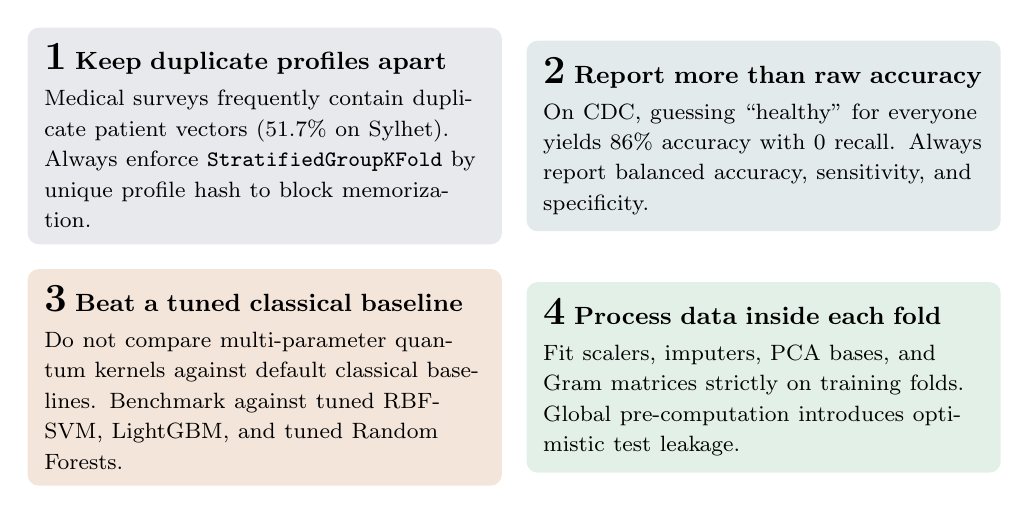
\begin{tikzpicture}[font=\small,
      card/.style={draw=none,rounded corners=4pt,text width=5.6cm,minimum height=2.1cm,inner sep=6pt,align=left}]
    \node[card,fill=qnavy!10](a){\textbf{\Large 1}\ \textbf{Keep duplicate profiles apart}\\[2pt]\footnotesize Medical surveys frequently contain duplicate patient vectors (51.7\% on Sylhet). Always enforce \texttt{StratifiedGroupKFold} by unique profile hash to block memorization.};
    \node[card,fill=qteal!12,right=0.3cm of a](b){\textbf{\Large 2}\ \textbf{Report more than raw accuracy}\\[2pt]\footnotesize On CDC, guessing ``healthy'' for everyone yields 86\% accuracy with 0 recall. Always report balanced accuracy, sensitivity, and specificity.};
    \node[card,fill=qamber!15,below=0.3cm of a](c){\textbf{\Large 3}\ \textbf{Beat a tuned classical baseline}\\[2pt]\footnotesize Do not compare multi-parameter quantum kernels against default classical baselines. Benchmark against tuned RBF-SVM, LightGBM, and tuned Random Forests.};
    \node[card,fill=qgreen!12,right=0.3cm of c](d){\textbf{\Large 4}\ \textbf{Process data inside each fold}\\[2pt]\footnotesize Fit scalers, imputers, PCA bases, and Gram matrices strictly on training folds. Global pre-computation introduces optimistic test leakage.};
  \end{tikzpicture}
  \pfoot{RBF = radial basis function; SVM = support vector machine; CDC = US Centers for Disease Control survey data; Sylhet = questionnaire survey; PCA = principal component analysis. Actionable standards to ensure reproducibility in clinical machine learning.}
\end{frame}

% ==============================================================================
% SLIDE 22: Conclusion
% ==============================================================================
\begin{frame}{Conclusion: Where Quantum ML Stands in Medicine}
  \begin{columns}[T]
    \column{0.52\textwidth}
      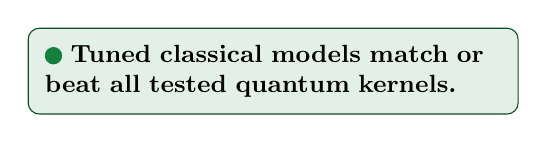
\begin{tikzpicture}[font=\small]
        \node[draw=qgreen!60!black,fill=qgreen!12,rounded corners,text width=5.8cm,inner sep=6pt]{\tlC{qgreen}\ \textbf{Tuned classical models match or beat all tested quantum kernels.}};
      \end{tikzpicture}\\[3pt]
      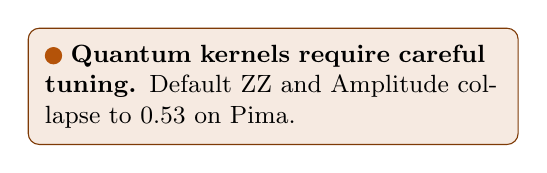
\begin{tikzpicture}[font=\small]
        \node[draw=qamber!70!black,fill=qamber!12,rounded corners,text width=5.8cm,inner sep=6pt]{\tlC{qamber}\ \textbf{Quantum kernels require careful tuning.} Default ZZ and Amplitude collapse to 0.53 on Pima.};
      \end{tikzpicture}\\[3pt]
      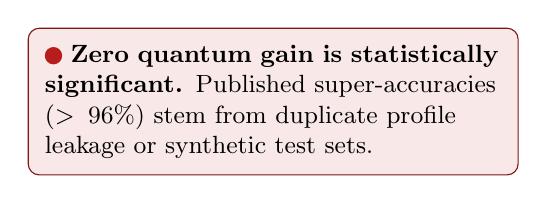
\begin{tikzpicture}[font=\small]
        \node[draw=qcrimson!70!black,fill=qcrimson!10,rounded corners,text width=5.8cm,inner sep=6pt]{\tlC{qcrimson}\ \textbf{Zero quantum gain is statistically significant.} Published super-accuracies ($>96\%$) stem from duplicate profile leakage or synthetic test sets.};
      \end{tikzpicture}

    \column{0.45\textwidth}
      \begin{block}{Scope \& Rigor of This Audit}
        \scriptsize
        \begin{itemize}
          \item 8 published architectures ported across 4 clinical diabetes cohorts ($N=520$ to $2{,}000$).
          \item Exact classical statevector simulation up to 8 qubits.
          \item 15 paired test folds per model with Holm FWER multiple-testing control.
          \item 100\% reproducible from open-source notebook suite.
        \end{itemize}
      \end{block}
      \begin{exampleblock}{Promising Niches for Medical Quantum Computing}
        \scriptsize Pivot away from low-dimensional tabular records toward physics-native problems: molecular dynamics, drug docking, and metabolic hypergraphs.
      \end{exampleblock}
  \end{columns}
  \pfoot{FWER = family-wise error rate; ZZ, Amplitude, Angle = quantum encodings; CDC = US Centers for Disease Control survey; Hosp 130 = hospital readmission registry. Code, notebooks, and verified datasets: repository \texttt{Adaptive-Quantum-Kernel-Selection}.}
\end{frame}

\end{document}
